\documentclass[aspectratio=1610]{beamer}
\graphicspath{{images/}}
%\usetheme{iclpt}
% slidenumber   (default true) turns on slide numbering
% titlepage     (default true) treats first slide as title slide (with IC/MRG logo)
% progressbar   (default false) turns on progress indicator at bottom of slide
% lighttheme    (default false) uses a 'light' theme with more subtle bottom bar
% sectionheader (default false) adds a top navigation bar (with section name)
% hashtag=STR   (default empty) adds a hashtag
% url=STR       (default mrg.doc.ic.ac.uk) add URL on bottom of slide
\usetheme[progressbar,lighttheme]{mrgpt}
\usepackage{booktabs}
\usepackage{colortbl}
\usepackage{roboto} % Use for fonts magic if using xelatex instead of pdflatex
\usepackage{tikz}
\usepackage{multirow}
\usepackage{xcolor}
\usepackage{scribble}
\usetikzlibrary{arrows,automata,backgrounds,calc,positioning,shapes}

\newcommand{\yes}{\textcolor{green!80!black}{\bfseries\checkmark}}

\title{Type-safe interactive web service generation from Scribble}
\author{Jonathan King, Nicholas Ng, Nobuko Yoshida}
\date{18 Dec 2018 --- ABCD project meeting}

\colorlet{gprot}{orange!80!black}
\colorlet{lprot}{blue}
\colorlet{efsm}{cyan}
\colorlet{proc}{purple}

\definecolor{javared}{rgb}{0.6,0,0} % for strings
\definecolor{javagreen}{rgb}{0.25,0.5,0.35} % comments
\definecolor{javapurple}{rgb}{0.5,0,0.35} % keywords
\definecolor{javadocblue}{rgb}{0.25,0.35,0.75} % javadoc
\lstdefinestyle{Java}{
  keywordstyle=\color{javapurple}\bfseries,
  stringstyle=\color{javared},
  commentstyle=\color{javagreen},
  morecomment=[s][\color{javadocblue}]{/**}{*/},
}

\begin{document}
\maketitle

\begin{frame}{The project}
  \begin{itemize}
    \item \textbf{Multiparty} Session Types for interactive web applications
    \item Scribble applied to PureScript \& WebSocket
      \begin{itemize}
        \item PureScript: strongly-typed functional language, compiles to JavaScript
        \item WebSocket: full-duplex communication from the browser
      \end{itemize}
    \item Encoding of local types/Endpoint FSMs as type classes and constraints
    \item Jonathan King's final year Master's project
    \item 8-months of term time work (concurrent with lectures)
  \end{itemize}
\end{frame}

\begin{frame}
  {Multiparty Session Types (MPST)}
  \begin{minipage}{0.60\linewidth}
    \resizebox{0.97\linewidth}{!}{
  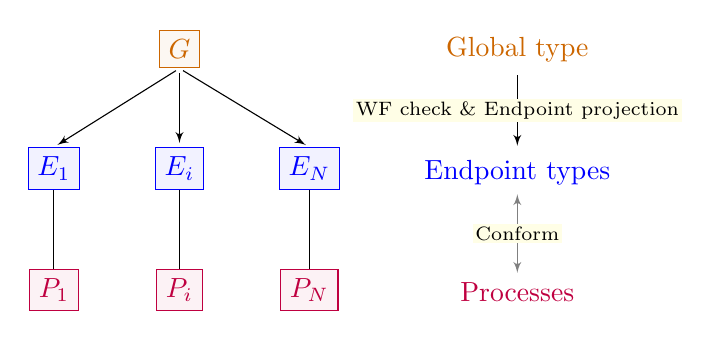
\begin{tikzpicture}[
      remember picture,
      box/.style={draw,minimum width=2},
      proj/.style={solid,>=latex',shorten <=1.5,shorten >=1.5},
      label/.style={inner sep=1,fill=yellow!10},
    ]
    \node (gt) [box,gprot,fill=gprot!5] {$G$};
    %
    \node (lt0) [below left=of gt,box,lprot,fill=lprot!5] {$E_1$};
    \node (lti) [below=of gt,box,lprot,fill=lprot!5] {$E_i$};
    \node (ltn) [below right=of gt,box,lprot,fill=lprot!5] {$E_N$};
    %
    \draw (lt0.north) edge [proj,<-] (gt.south);
    \draw (lti.north) edge [proj,<-] (gt.south);
    \draw (ltn.north) edge [proj,<-] (gt.south);
    %
    \node (p0) [below=of lt0,box,proc,fill=proc!5] {$P_1$};
    \node (pi) [below=of lti,box,proc,fill=proc!5] {$P_i$};
    \node (pn) [below=of ltn,box,proc,fill=proc!5] {$P_N$};
    %
    \draw (p0.north) edge (lt0.south);
    \draw (pi.north) edge (lti.south);
    \draw (pn.north) edge (ltn.south);
    %
    \node (gtext) [right=3 of gt,gprot] {Global type};
    \node (ltext) [below=of gtext,lprot] {Endpoint types}
     edge [proj,<-]
     node [midway,label]
      {\scriptsize WF check \& Endpoint projection} (gtext);
    \node (ptext) [below=of ltext,proc] {Processes}
     edge [<->,draw=gray,>=latex']
     node (lplabel) [midway,label]
       {\scriptsize Conform} (ltext);
    %
  \end{tikzpicture}
  }% resizebox
  \vspace{4ex}
  \end{minipage}
  \begin{minipage}{0.38\linewidth}
  Specify
  \begin{itemize}
    \item \textcolor{gprot}{Global msg-passing protocol}
  \end{itemize}
  Implement
  \begin{itemize}
    \item \textcolor{proc}{Endpoint processes}
  \end{itemize}
  Guarantees
  \begin{itemize}
    \item[\yes] Communication safety
    \item[\yes] Deadlock freedom
    \item[\yes] Protocol fidelity
  \end{itemize}
  \end{minipage}

  Verification techniques for \tikz[remember picture,overlay,baseline]{
    \node [anchor=base,xshift=2.5em,inner sep=1,fill=yellow!10] {conformance}
     edge [densely dotted,out=0,in=0,shorten <=0.5em] (lplabel.east);}
  \begin{itemize}
    \item Static type checking against implementation
    \item Runtime monitoring
    \item APIs/code generation from session types
  \end{itemize}
\end{frame}

\begin{frame}[fragile]{Implementations and applications of MPST using Scribble}
  \resizebox{0.98\linewidth}{!}{%
  \begin{tikzpicture}[
      box/.style={draw,minimum width=2},
      proj/.style={solid,>=latex',shorten <=1.5,shorten >=1.5},
      label/.style={inner sep=1,fill=yellow!10},
      example/.style={rectangle split,rectangle split parts=2,rectangle split part align={left,left},inner sep=0},
      st/.style={state,minimum size=0pt,inner sep=3,efsm},
      tr/.style={bend right,<-,>=latex',thick,efsm},
      every initial by arrow/.style={efsm},
    ]
    \node (g) [box,gprot,fill=gprot!5] {$G$};
    %
    \node (l0) [below left=1.5 and 1 of g,box,lprot,fill=lprot!5] {$E_1$};
    \node (li) [below=1.5 of g,box,lprot,fill=lprot!5] {$E_i$};
    \node (ln) [below right=1.5 and 1 of g,box,lprot,fill=lprot!5] {$E_N$};
    %
    \draw (l0.north) edge [proj,<-] (g.south);
    \draw (li.north) edge [proj,<-] (g.south);
    \draw (ln.north) edge [proj,<-] (g.south);
    %
    \node (e0) [below=1 of l0,efsm] {$EFSM_1$} edge [densely dotted] (l0);
    \node (ei) [below=1 of li,efsm] {$EFSM_i$} edge [densely dotted] (li);
    \node (en) [below=1 of ln,efsm] {$EFSM_N$} edge [densely dotted] (ln);
    %
    \draw(e0) -- ($(e0)+(0,-1.5)$);
    \draw(ei) -- ($(ei)+(0,-1.5)$);
    \draw(en) -- ($(en)+(0,-1.5)$);
    %
    \fill [proc!5] ($(e0.west)+(-0.2,-1.5)$) rectangle ($(en.east)+(0.2,-2.5)$)
    node [midway,proc] {Language \& runtime support};

    \node (gtext2) [right=4 of g,gprot] {Global protocol};
    \node (ltext2) [below=1.5 of gtext2,lprot] {Endpoint protocols}
     edge [proj,<-]
     node [midway,label]
      {\scriptsize WF check \& Endpoint projection} (gtext2);
    \node (etext2) [below=1 of ltext2,efsm] {Endpoint FSMs}
     edge [densely dotted,<-]
     node [midway,label]
      {\scriptsize Translate} (ltext2);
    \node (ptext2) [below=of etext2,proc] {APIs for endpoint programming}
     edge [<-,draw=gray]
     node [midway,inner sep=0.5,fill=yellow!10]
      {\scriptsize Generate} (etext2);
      \node (gex) [right=2 of gtext2,example] {
        \textcolor{gprot}{\small Global Scribble protocol}
        \nodepart{two}
        \lstinputlisting[language=Scribble,style=Scribble,basicstyle=\tiny\ttfamily]{./code/scribble-global.scr}
      };
      \node (lex) [below=of gex.south west,anchor=north west,example] {
        \textcolor{lprot}{\small Endpoint Scribble protocol S}
        \nodepart{two}
        \lstinputlisting[language=Scribble,style=Scribble,basicstyle=\tiny\ttfamily]{./code/scribble-local.scr}
      };
      \node (eex) [below=of lex.south west,anchor=north west,efsm] {\small Endpoint FSM for \texttt{S}};
      \node (q0) [initial,initial text={},st,below=0.5 of eex.south,anchor=north west,xshift=-2em] {};
      \node (q1) [st,right=of q0] {}
       edge [tr]
       node [midway,above] {\tiny $c!$\texttt{int}} (q0);
      \node (q2) [accepting,st,right=of q1] {}
       edge [tr]
       node [midway,above] {\tiny $c?$\texttt{bool}} (q1);
      %
      \node (pex) [below=2 of eex.south west,anchor=north west,example] {
        \textcolor{proc}{\small Endpoint APIs (for users), e.g.~Java}
        \nodepart{two}
        \lstinputlisting[language=Java,basicstyle=\scriptsize\ttfamily,style=Java]{./code/p_s.java}
      };
      \draw ($(gex.south west)+(3em,0)$)
       edge [proj,->]
       node [midway,label] {\scriptsize Project} ($(lex.north west)+(3em,0)$);
      \draw ($(lex.south west)+(3em,0)$)
       edge [densely dotted,->]
       node [midway,label] {\scriptsize Translate} ($(eex.north west)+(3em,0)$);
      \draw ($(eex.south west)+(3em,-1)$)
       edge [->,draw=gray]
       node [midway,label] {\scriptsize Generate} ($(pex.north west)+(3em,0)$);
    \end{tikzpicture}
  } % resizebox
\end{frame}

\begin{frame}{Implementations and applications of MPST using Scribble}

  Some example uses:

  \begin{table}
  \begin{tabular}{lll}
    \toprule
    & Language & Transports\\
    \midrule
    Hybrid session verification (FASE'16)  & \multirow{2}{*}{Java} &\multirow {2}{*}{\small TCP, SSL/TCP, HTTP}\\
    Explicit connection actions (FASE'17)  &      &\\
    Typestate generation (SCP, 2017)       & Java &\small Java methods\\
    Linear decomposition (ECOOP'17)        & Scala&\small TCP, shared mem., Akka actors\\
    Session Type Provider (CC'18)          & F\#  &\small TCP\\
    Role-parametric MPST (POPL'19)\footnote{Talk this afternoon} & Go   &\small TCP, shared mem.\\
    \bottomrule
  \end{tabular}
  \end{table}
  \uncover<2>{
    \begin{itemize}
      \item All target desktop/distributed applications
      \item Can we apply it to web applications?
    \end{itemize}
  }
\end{frame}

\begin{frame}{Example: Scribble playground}{}
  \begin{minipage}{0.55\linewidth}
    Web-based interface to the Scribble tool
    \begin{itemize}
      \item \textbf{Check} protocols
      \item \textbf{Project} protocol to endpoint protocols
      \item \textbf{Generate FSM} from Scribble protocols
    \end{itemize}
    \vspace{3ex}
    \textit{Communicates} with server to execute Scribble
    \\[3ex]
    {\footnotesize (Similar web-based \textit{playground} exist for Go, Rust, etc.)}
  \end{minipage}
  \begin{minipage}{0.43\linewidth}
    \quad
    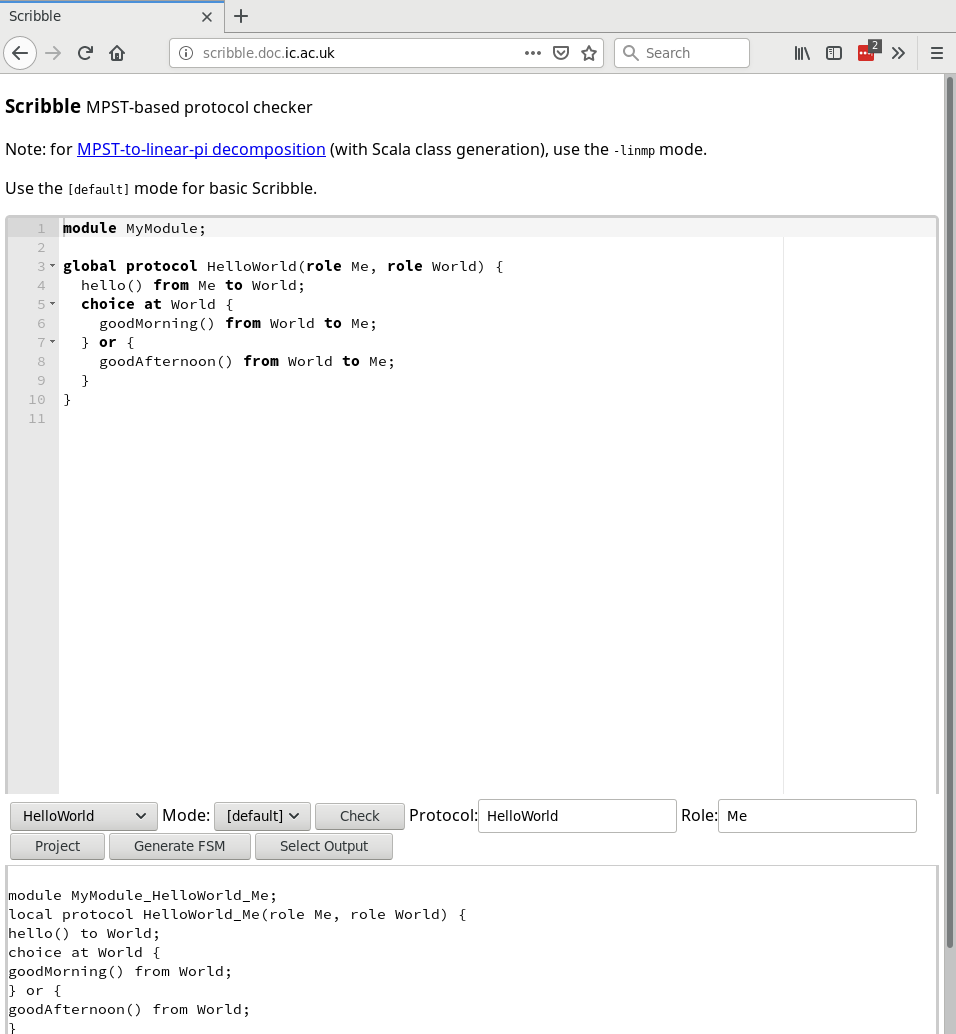
\includegraphics[width=\linewidth]{scribble-playground}
  \end{minipage}
\end{frame}

\begin{frame}{Scribble-based API generation for the web}
  \begin{table}
  \begin{tabular}{lll}
    \toprule
    & Language & Transports\\
    \midrule
    Hybrid session verification (FASE'16)  & \multirow{2}{*}{Java} &\multirow {2}{*}{\small TCP, SSL/TCP, HTTP}\\
    Explicit connection actions (FASE'17)  &      &\\
    Typestate generation (SCP, 2017)       & Java &\small Java methods\\
    Linear decomposition (ECOOP'17)        & Scala&\small TCP, shared mem., Akka actors\\
    Session Type Provider (CC'18)          & F\#  &\small TCP\\
    Role-parametric MPST (POPL'19)         & Go   &\small TCP, shared mem.\\
    \rowcolor{yellow!10} \textbf{This work's aim}  & \textbf{JavaScript} &\small \textbf{WebSocket} \\
    \bottomrule
  \end{tabular}
  \end{table}

  \textbf{Challenge}: JavaScript not statically typed
\end{frame}

\begin{frame}{PureScript}{A strongly-typed functional programming language that compiles to JavaScript}
  From PureScript homepage:
  \begin{itemize}
    \item \alert<2>{Compile to readable JavaScript} and reuse existing JavaScript code easily
    \item An extensive collection of libraries for development of web applications, web servers, apps and more
    \item Excellent tooling and editor support with instant rebuilds
    \item An active community with many learning resources
    \item Build real-world applications using functional techniques and expressive types, such as:
      \begin{itemize}
        \item Algebraic data types and pattern matching
        \item \alert<2>{Row polymorphism} and extensible records
        \item Higher kinded types
        \item \alert<2>{Type classes with functional dependencies}
        \item Higher-rank polymorphism
      \end{itemize}
  \end{itemize}
\end{frame}

\begin{frame}{PureScript code generation}
  From the EFSM, PureScript types are generated:
  \begin{itemize}
    \item Each \textbf{state} is a type
    \item Each \textbf{transition} is a type class instance
  \end{itemize}

  The core type classes:
  \begin{itemize}
    \item Send: message send
    \item Recv: message receive
    \item Select: selection (receive label)
    \item Branch: branching (send label)
  \end{itemize}
\end{frame}

\begin{frame}{Multi-parameter type classes and functional dependencies}
\end{frame}

\begin{frame}{Scribble playground}
\end{frame}

\begin{frame}{Summary}
  \begin{description}
    \item [\bf Specify] \textcolor{gprot}{global protocol} in Scribble
    \item [Project] \textcolor{gprot}{global protocol} into \textcolor{lprot}{local protocols}
    \item [Translate] \textcolor{lprot}{local protocol} to \textcolor{efsm}{EFSM}
    \item [Generate] PureScript type constraints of protocol from \textcolor{efsm}{EFSM}
    \item [\bf Write] \textcolor{proc}{web application} endpoint in PureScript
    \item [\bf Run] type-safe web application
  \end{description}
\end{frame}
\end{document}
